\documentclass[11pt]{article}

\usepackage[margin=2.5cm]{geometry}
\usepackage{graphicx}
\usepackage{amsmath}
\usepackage{float}
\usepackage{hyperref}

\title{Random Leakages}
\author{}
\date{\today}

% allow more figures to pack onto one page (default limits are conservative
% for a figure-heavy document like this one)
\renewcommand{\topfraction}{0.9}
\renewcommand{\textfraction}{0.05}
\renewcommand{\floatpagefraction}{0.8}
\setcounter{topnumber}{5}
\setcounter{totalnumber}{5}

\begin{document}
\maketitle

\section*{Overview}

The runs collected here all use the single-influx-resource minimal MiCRM model
(\texttt{scripts/single\_influx.jl}): a well-mixed community is sampled, its
steady state is found by integrating the ODEs, and the outcome is classified as
\emph{extinct} (all consumers die out), \emph{stable} (a well-mixed coexistence
steady state that also survives a linear stability check against spatial
perturbations at a range of wavenumbers), or \emph{unstable} (the steady state
is only stable when well-mixed, and a spatial instability is found). This is
repeated many times over a grid of the normalized energy supply rate $K$ and
the shape of the per-strain leakage fraction, which is drawn from a Beta
distribution for each sampled community. The two runs below differ only in how
that Beta distribution is parametrized and swept.

\section{\texttt{single\_influx\_randl2} / \texttt{main2}}

\paragraph{Data.} Directory: \texttt{cluster\_env/runs/single\_influx\_randl2},
generated by \texttt{main2()} in that directory's \texttt{base.jl} (submitted
via \texttt{job2.slurm}).

\paragraph{Description.} This run parametrizes the leakage Beta distribution
by a target \emph{mean} and a \emph{spread factor}: the spread factor is the
standard deviation expressed as a fraction of the largest value that keeps the
distribution unimodal for that mean (so a factor near~0 is a near-deterministic
leakage value, and~1 is the widest unimodal spread possible). The mean is swept
over 15 values, non-linearly rescaled to concentrate samples near a leakage of~1
(the biologically relevant high-leakage regime), and the spread factor is swept
over 4 values, $\{0.0009,\ 0.045,\ 0.156,\ 0.333\}$, from essentially fixed
leakage up to a third of the maximum non-bimodal spread. $K$ is swept over 30
log-spaced values from $1$ to $\sim\!3160$. With 150 repeats per
$(K,\text{mean},\text{spread})$ combination this is 270{,}000 individual runs.

\begin{figure}[H]
    \centering
    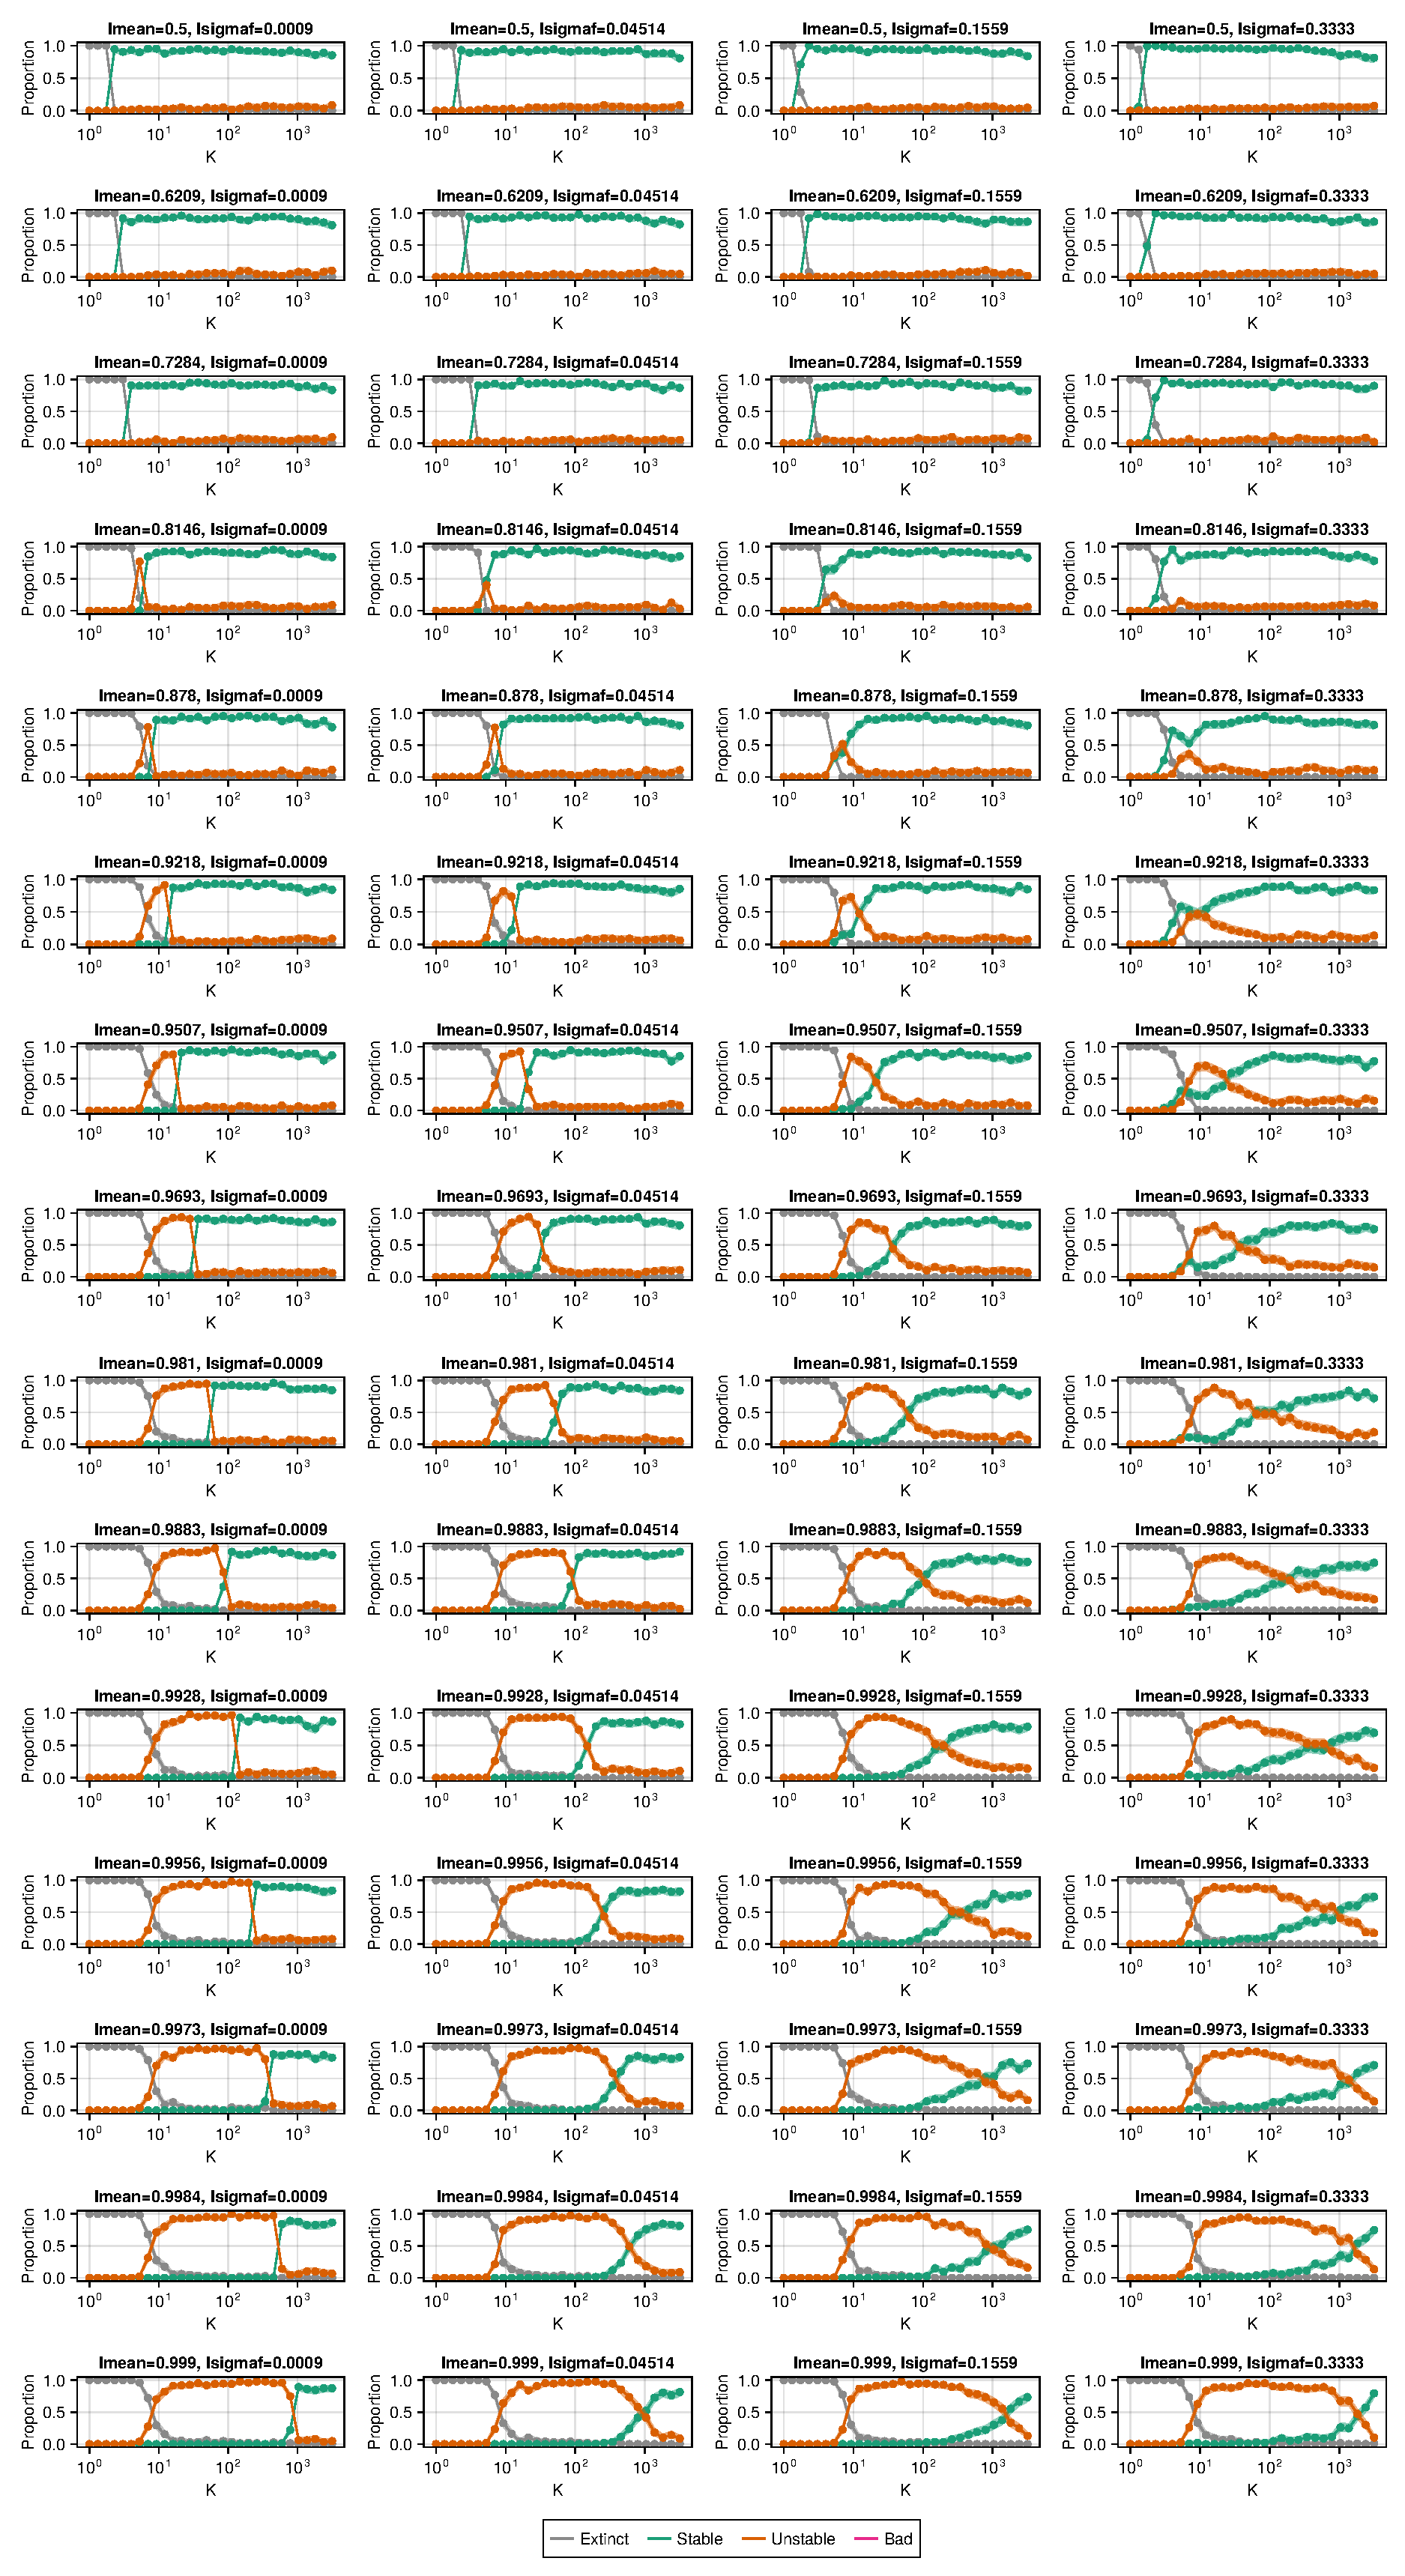
\includegraphics[width=\textwidth,height=0.85\textheight,keepaspectratio]{../../cluster_env/runs/single_influx_randl2/main2_plots/proportions.pdf}
    \caption{Proportion of extinct/stable/unstable outcomes vs.\ $K$, tiled by
    mean leakage (rows) and spread factor (columns).}
\end{figure}

\begin{figure}[H]
    \centering
    \begin{minipage}{0.76\textwidth}
        \centering
        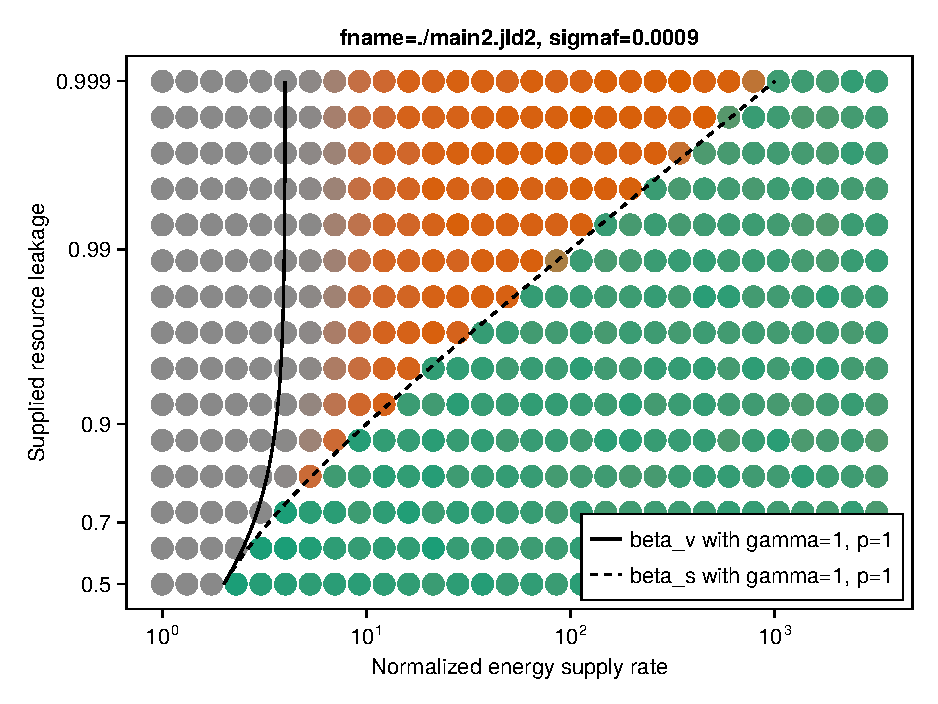
\includegraphics[width=0.49\linewidth]{../../cluster_env/runs/single_influx_randl2/main2_plots/main2_sigmai_1.pdf}
        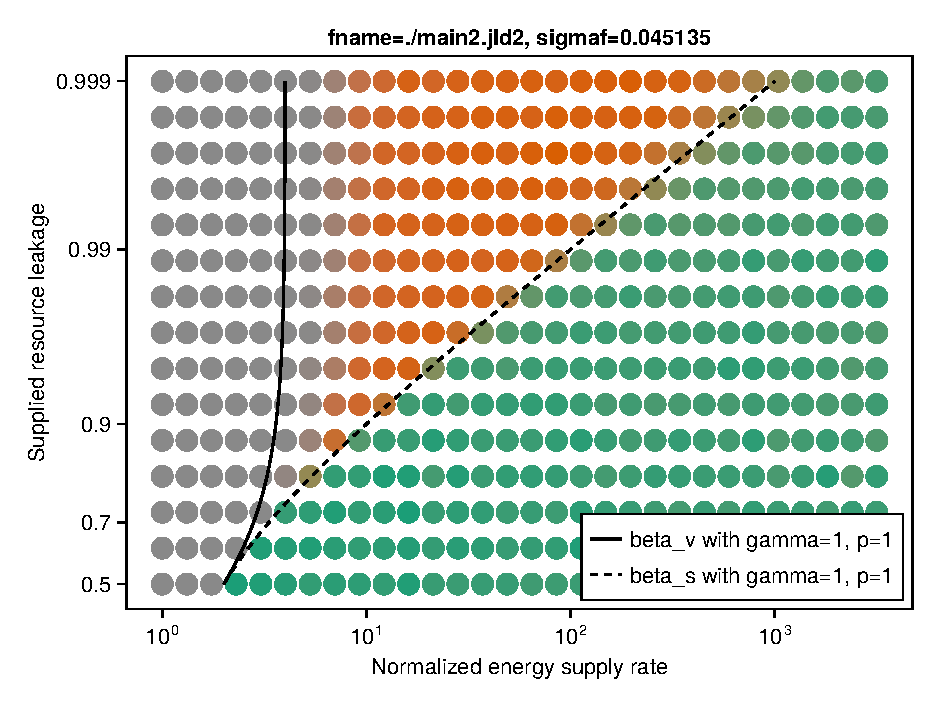
\includegraphics[width=0.49\linewidth]{../../cluster_env/runs/single_influx_randl2/main2_plots/main2_sigmai_2.pdf}\\
        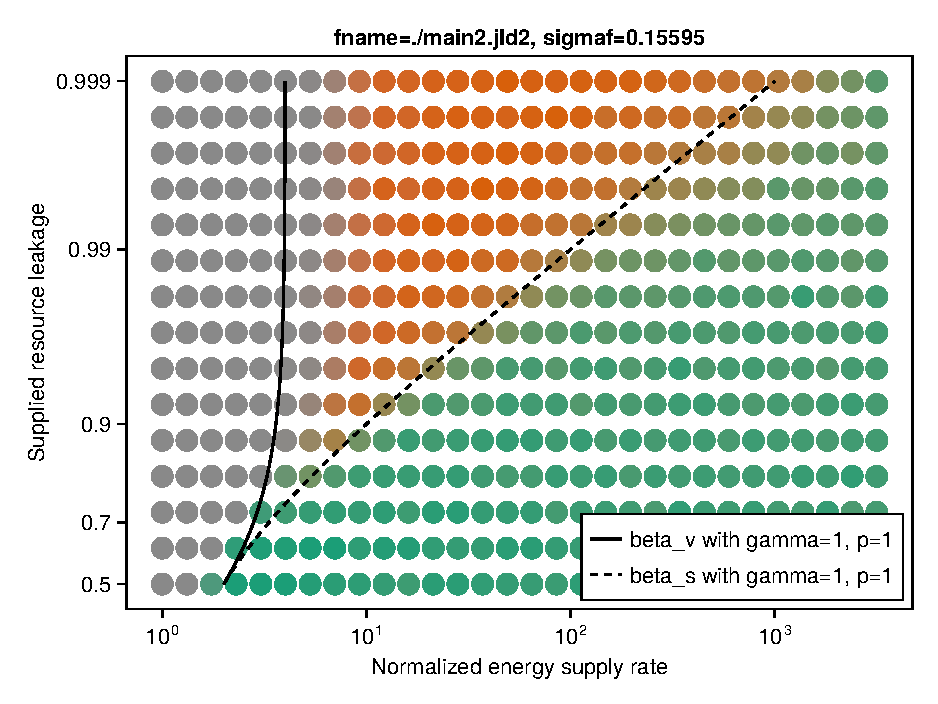
\includegraphics[width=0.49\linewidth]{../../cluster_env/runs/single_influx_randl2/main2_plots/main2_sigmai_3.pdf}
        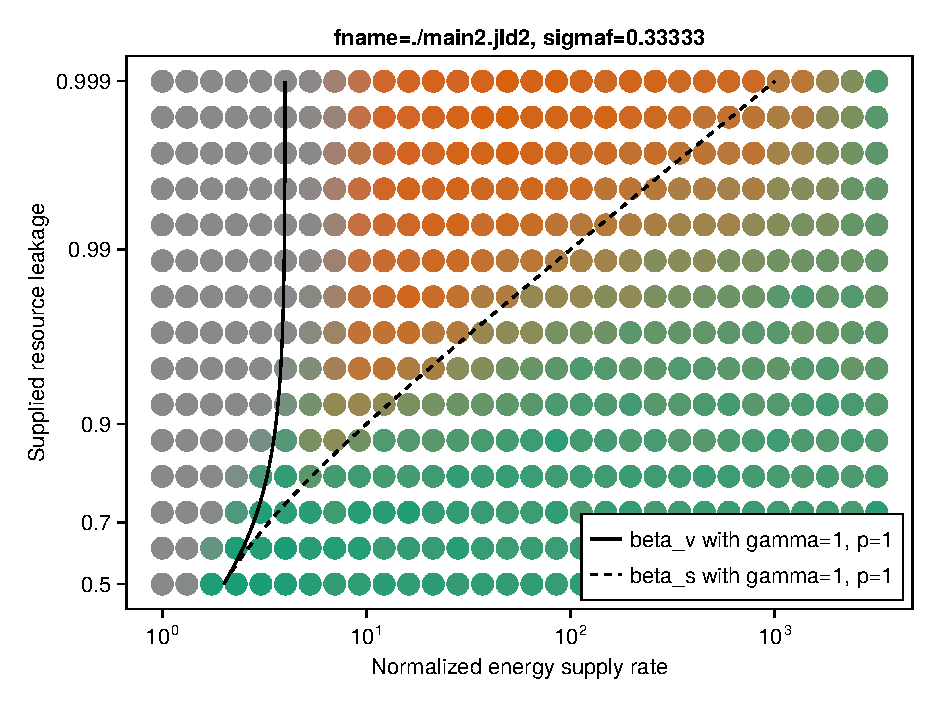
\includegraphics[width=0.49\linewidth]{../../cluster_env/runs/single_influx_randl2/main2_plots/main2_sigmai_4.pdf}
    \end{minipage}%
    \hfill
    \begin{minipage}{0.2\textwidth}
        \centering
        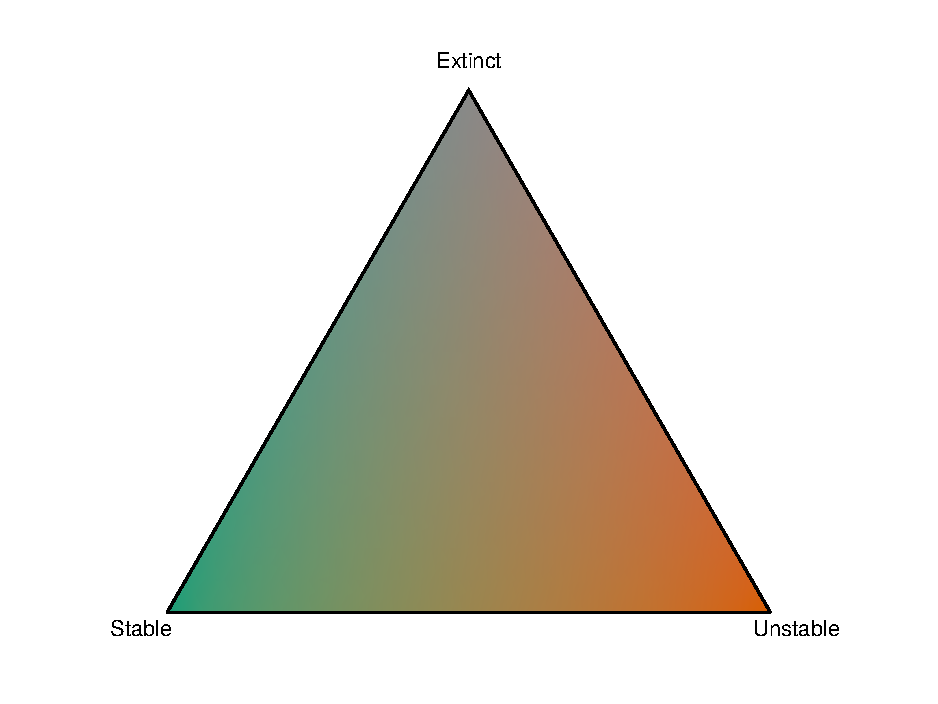
\includegraphics[width=\linewidth]{../../figures2/fig2/outcomes_colormap_fullsize.pdf}
    \end{minipage}
    \caption{Outcome phase diagram ($K$ vs.\ leakage, coloured by the ternary
    extinct/stable/unstable proportion), one panel per spread factor index
    (1 to 4, narrowest to widest), with the colour legend on the right.}
\end{figure}

\begin{figure}[H]
    \centering
    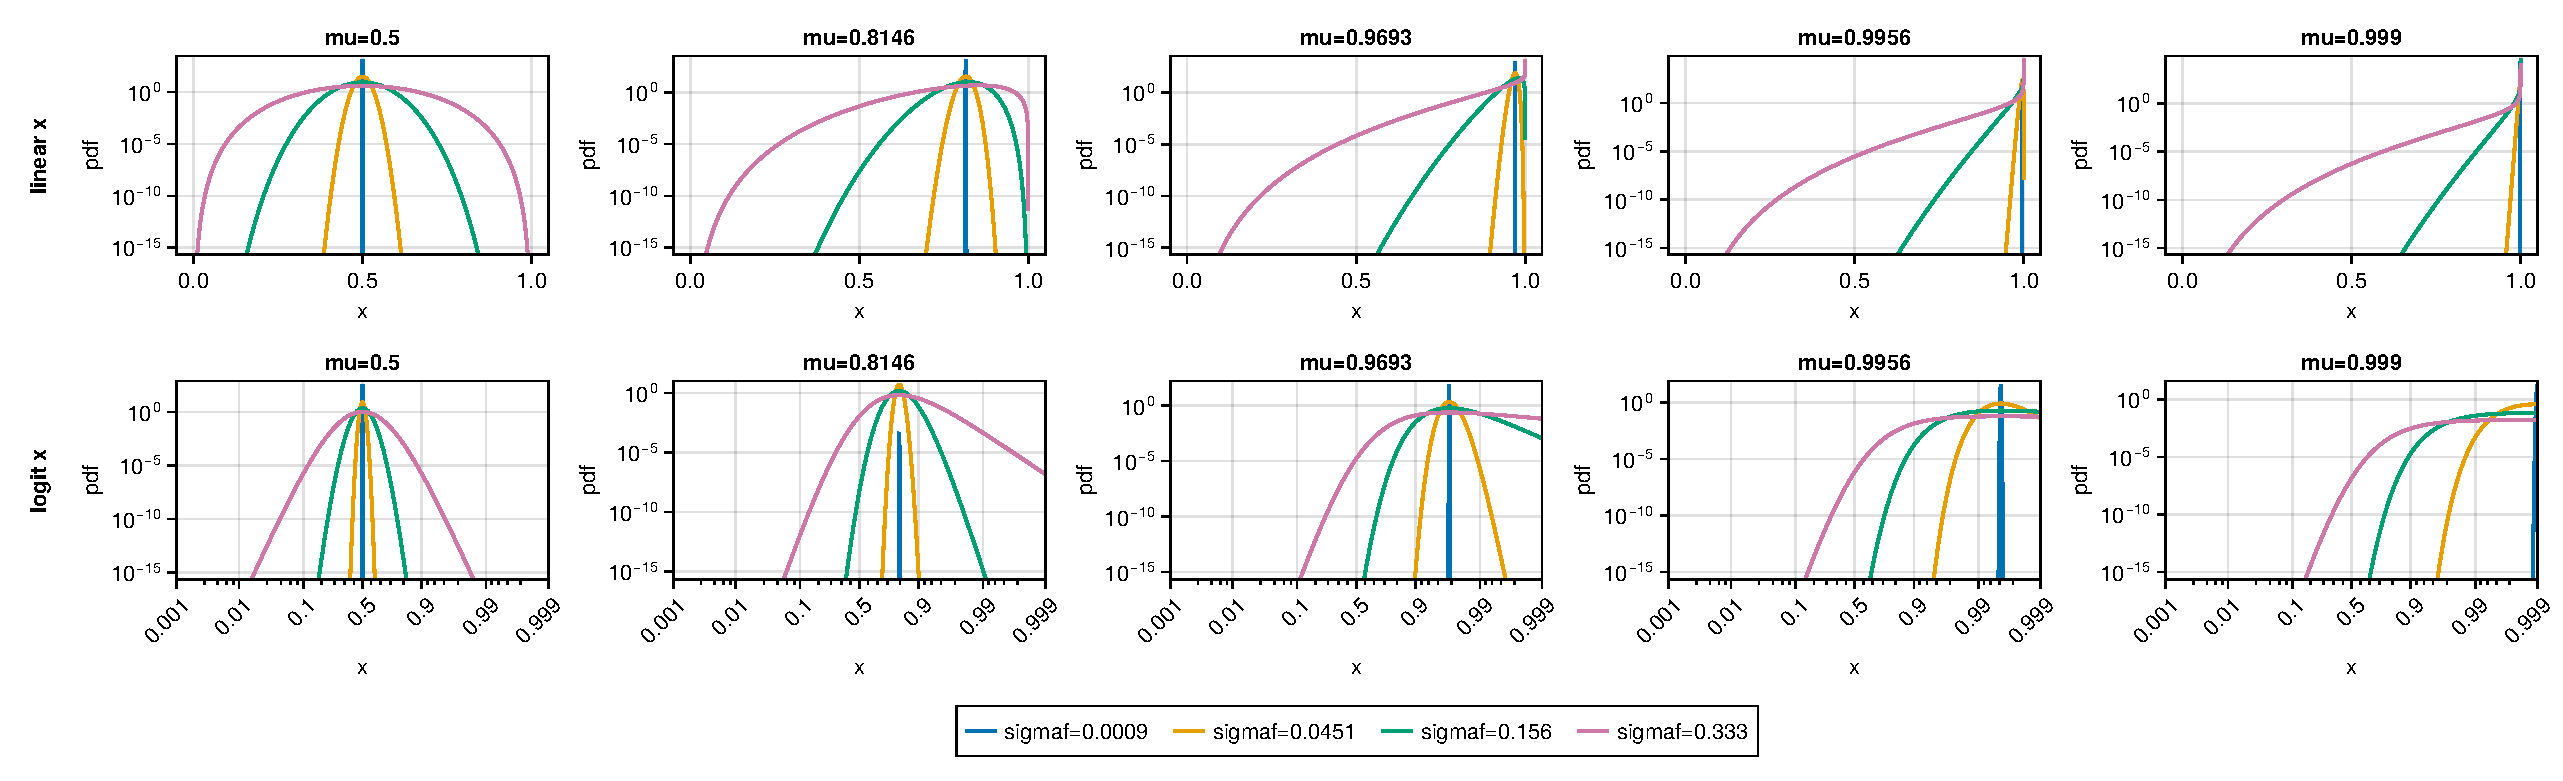
\includegraphics[width=\textwidth]{../../cluster_env/runs/single_influx_randl2/main2_plots/beta_dists.pdf}
    \caption{The sampled leakage distribution, $\mathrm{Beta}(\mu,
    \sigma_f \cdot \sigma_{\max}(\mu))$, for five representative mean-leakage
    values spread across the swept range (including the smallest and largest),
    each panel showing all four spread factors $\sigma_f$.}
\end{figure}

\clearpage
\section{\texttt{single\_influx\_randl3} / \texttt{main1}}

\paragraph{Data.} Directory: \texttt{cluster\_env/runs/single\_influx\_randl3},
generated by \texttt{main1()} in that directory's \texttt{base.jl} (submitted
via \texttt{job1.slurm}).

\paragraph{Description.} This run instead parametrizes the leakage Beta
distribution directly by its native shape parameters $\alpha$ and $\beta$,
each swept over the same 6 dyadic values $\{0.5, 1.32, 3.48, 9.19, 24.25, 64\}$
(all $36$ combinations), which covers everything from U-shaped/bimodal
distributions ($\alpha,\beta < 1$) through to sharply peaked, nearly
deterministic ones ($\alpha,\beta \gg 1$), including both symmetric
($\alpha=\beta$, centred at a leakage of $0.5$) and skewed combinations biased
towards low or high leakage. $K$ is swept over 50 log-spaced values from $1$ to
$\sim\!3160$. With 150 repeats per $(K,\alpha,\beta)$ combination this is also
270{,}000 individual runs.

\begin{figure}[H]
    \centering
    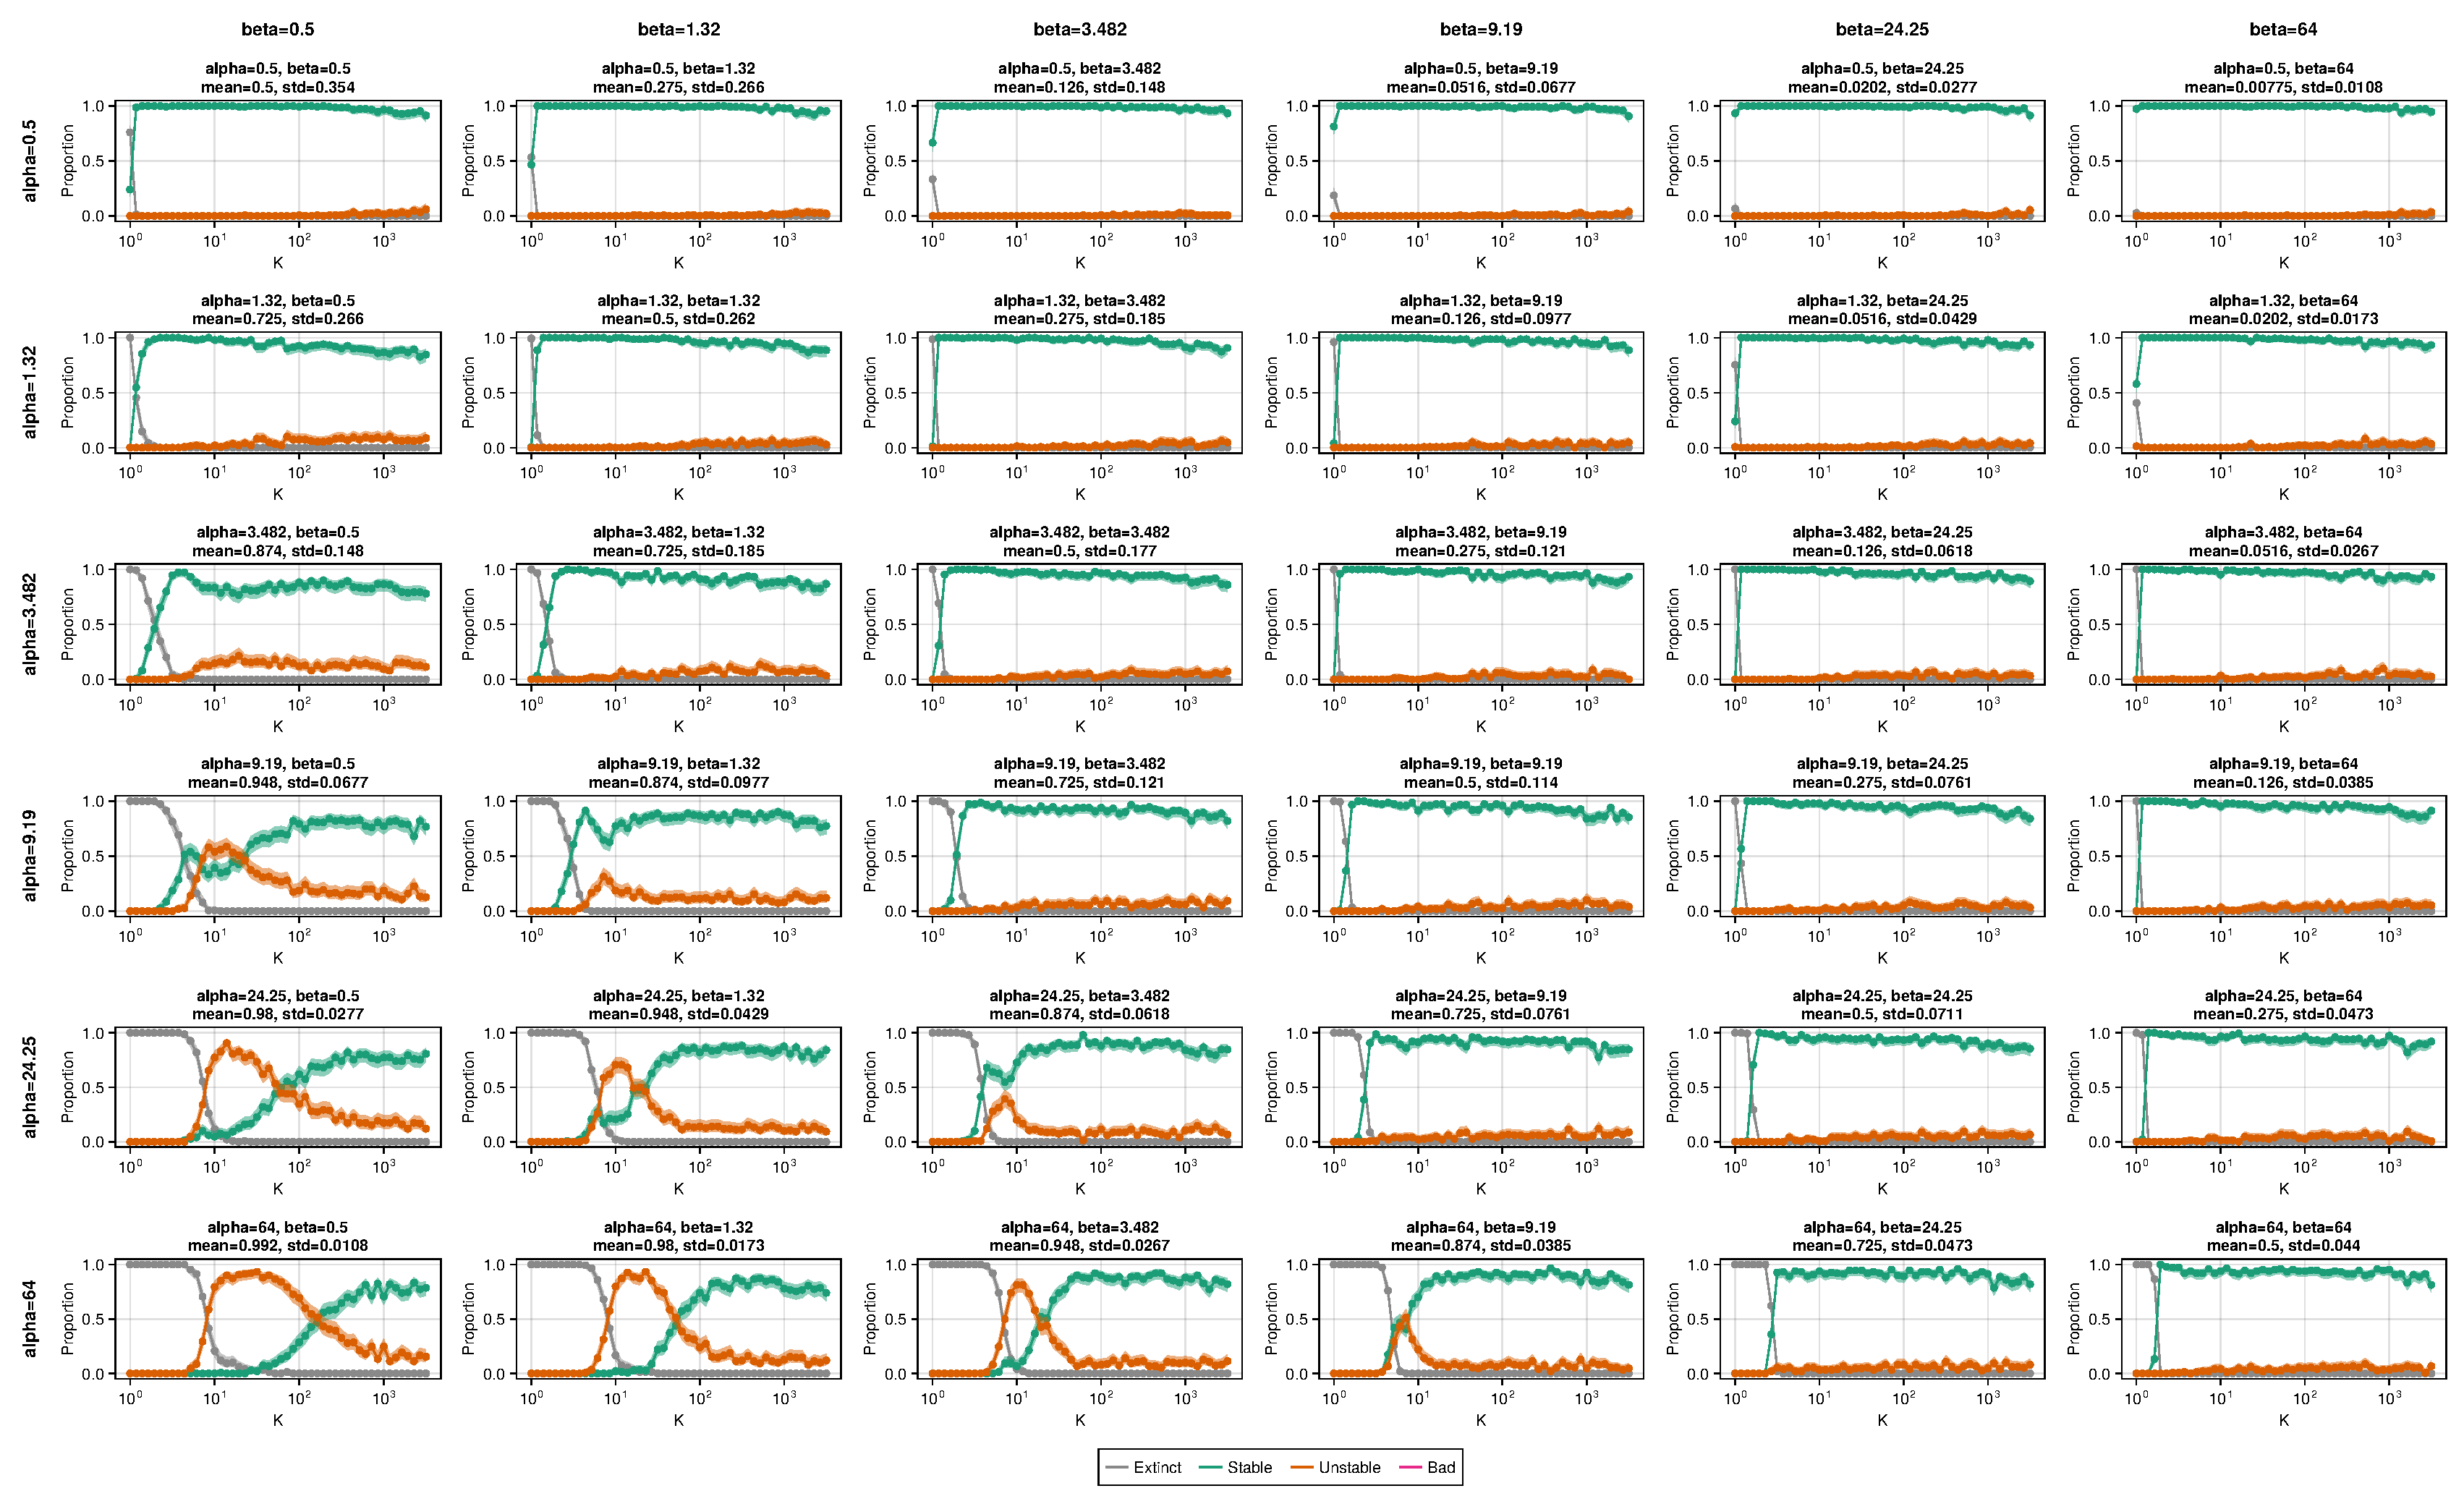
\includegraphics[width=\textwidth,height=0.85\textheight,keepaspectratio]{../../cluster_env/runs/single_influx_randl3/main1_plots/proportions.pdf}
    \caption{Proportion of extinct/stable/unstable outcomes vs.\ $K$, tiled by
    $\alpha$ (rows) and $\beta$ (columns).}
\end{figure}

\begin{figure}[H]
    \centering
    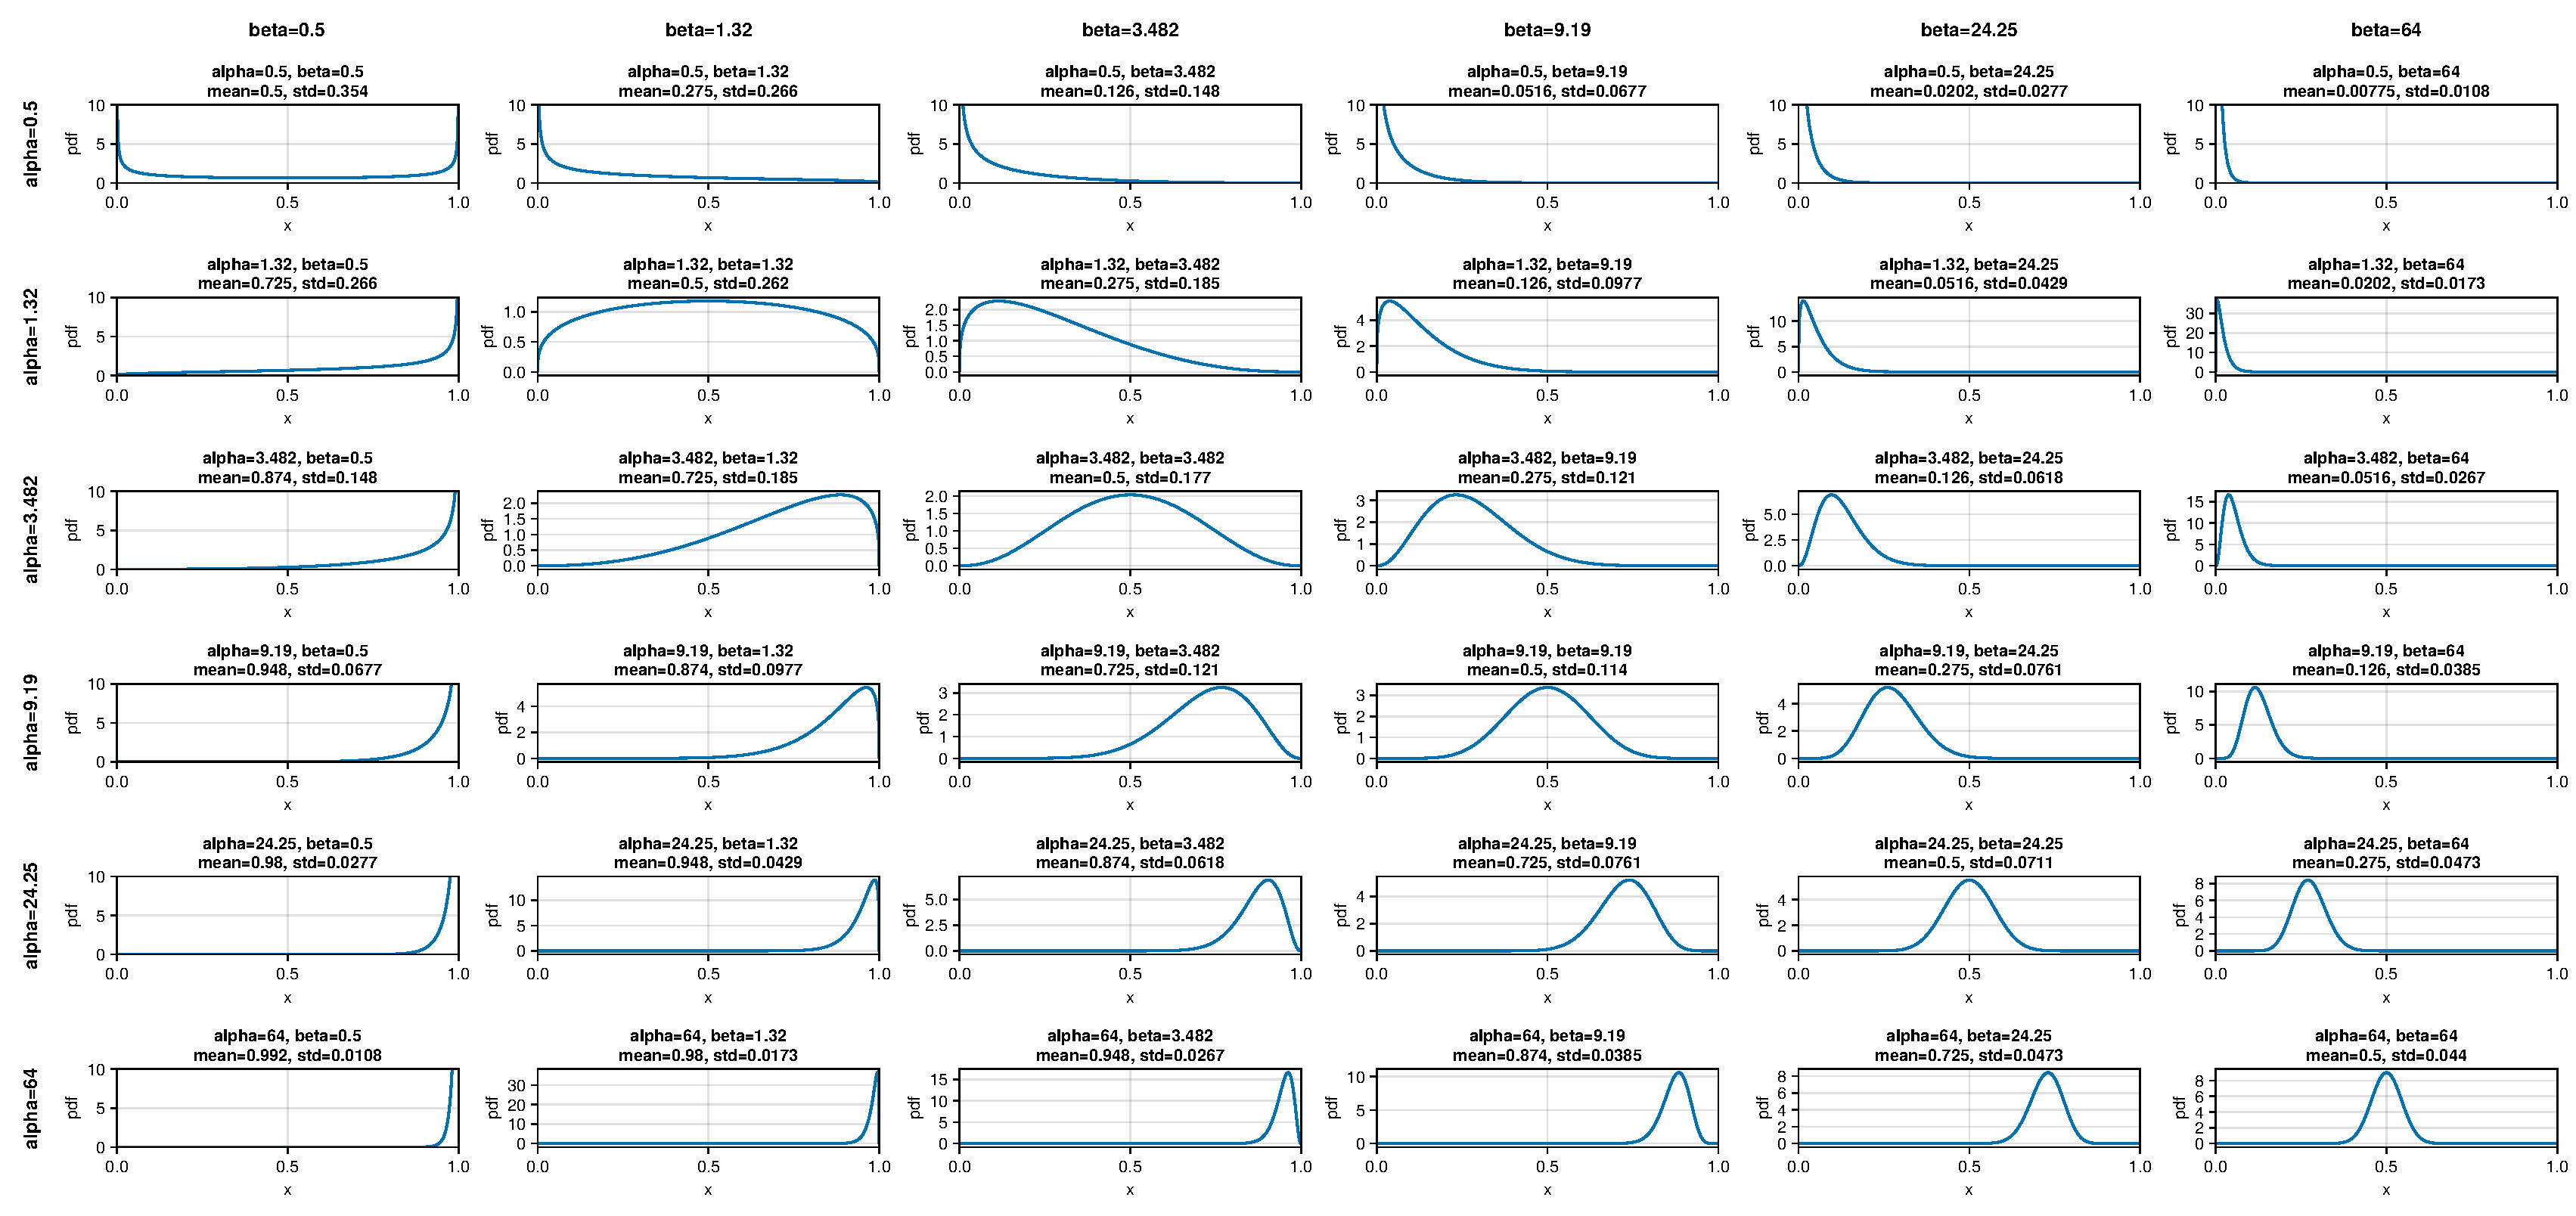
\includegraphics[width=\textwidth,height=0.85\textheight,keepaspectratio]{../../cluster_env/runs/single_influx_randl3/main1_plots/distributions.pdf}
    \caption{The sampled leakage distribution, $\mathrm{Beta}(\alpha,\beta)$,
    at each grid position -- directly comparable panel-for-panel with the
    outcome proportions above.}
\end{figure}

\end{document}
